\section{Geometry of 3D Reconstruction}
\label{s:fundamental}
In order to understand the purpose of the fundamental and essential matrix, we first describe epipolar geometry. Epipolar geometry captures the intrinsic projective geometry between two cameras views, which only depends on the internal parameters of the camera and relative positions of the two views. The fundamental matrix contains this information, and from the fundamental matrix, we can derive the essential matrix, which gives us the relative position and orientation of the two camera views. From that, we can derive the actual 3d points of the points in both views.

\subsection{Epipolar Geometry}
In our project, we take two uncalibrated pictures of the same object but from different views. Epipolar geometry gives us a relationship between these images.
\begin{figure}[H]
\begin{center}
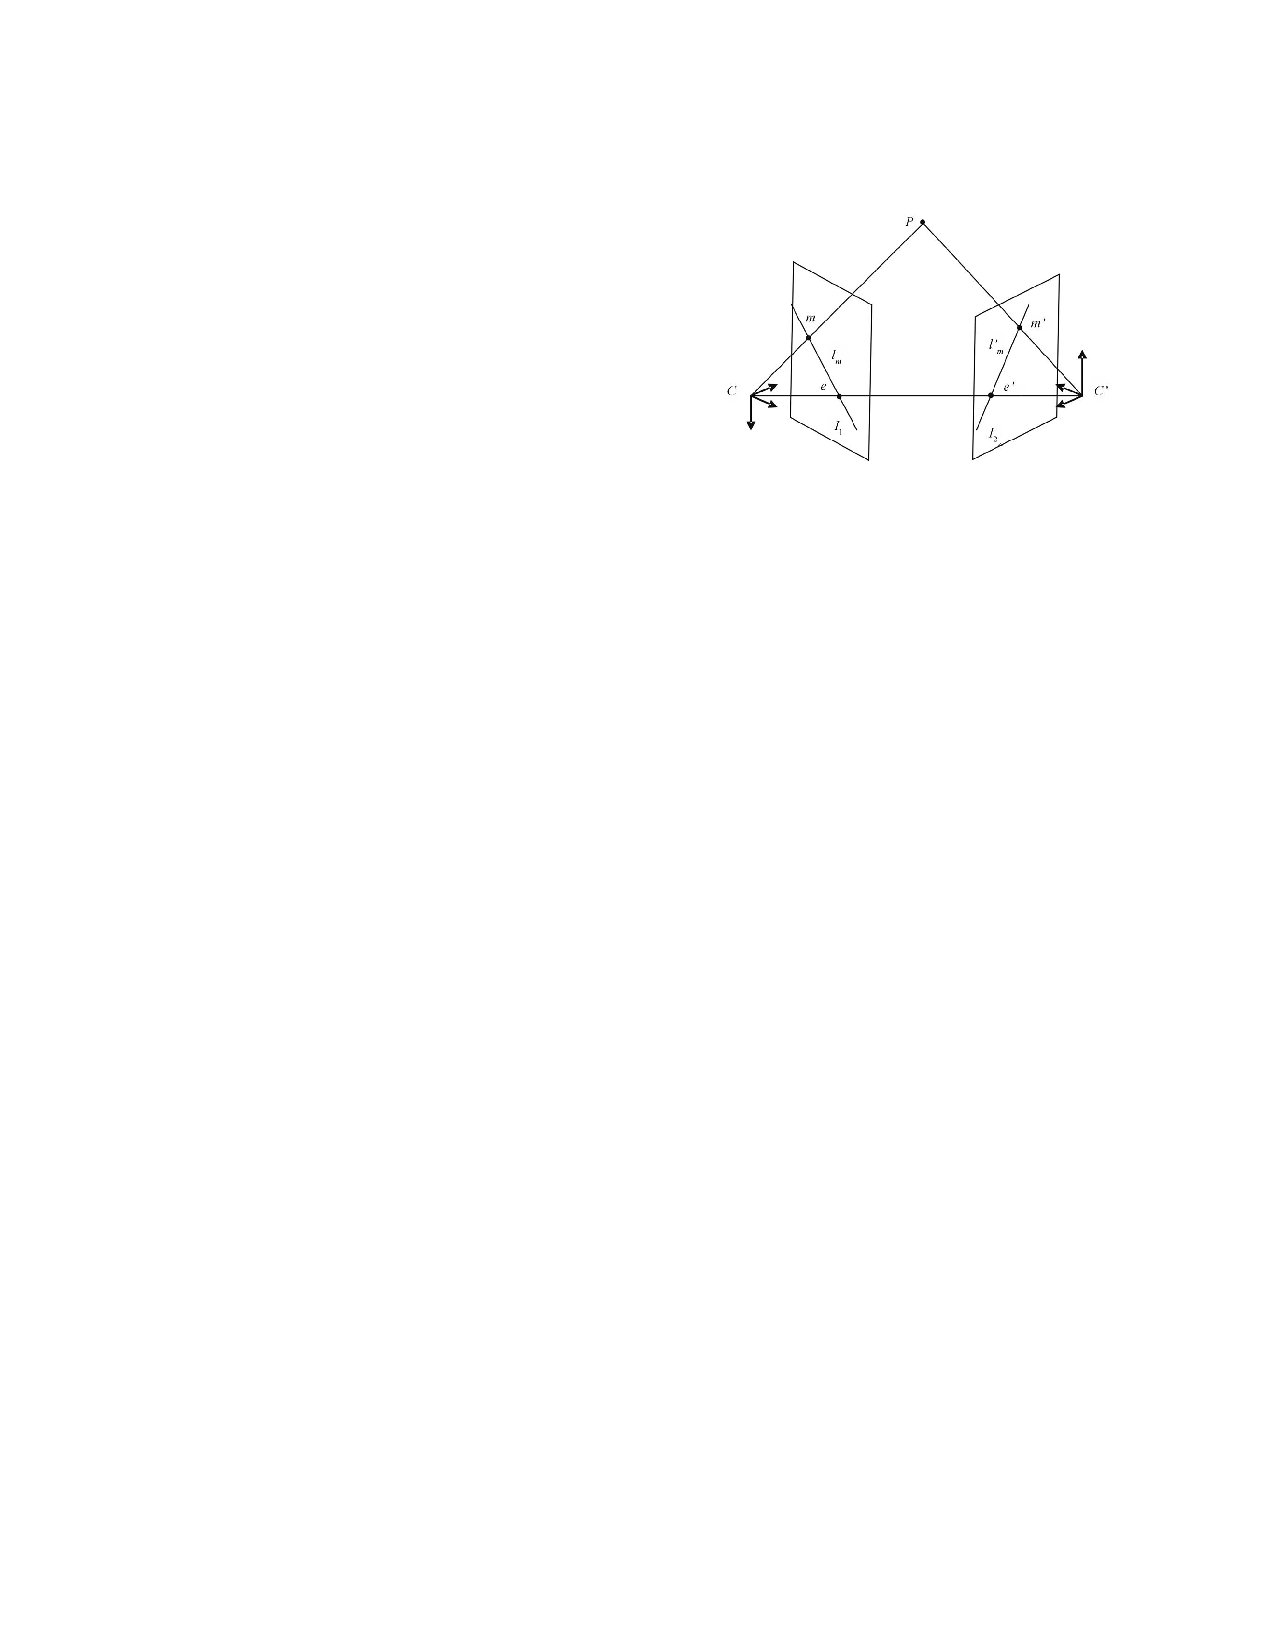
\includegraphics[width=0.9\linewidth]{figures/epipolar.pdf}
\end{center}
\caption{Epipolar geometry of two images from different views.}
\label{epipolar_pic}
\end{figure}

Figure~\ref{epipolar_pic} illustrates the relevant epipolar geometry. $I_1$ and $I_2$ are the images planes and $C$ and $C'$ represent the optical center of the camera from different views. $m$ and $m'$ represent $P$ projected onto $I_1$ and $I_2$ respectively. $e$ and $e'$ represent the epipoles, which are the intersections of the image planes with the line connects the camera centers. $l_m$ and $l_m'$ are the epipolar lines, which is where the epipolar plane intersects the image plane. It is important to note that $m$ and $m'$ lie on the $l_m$ and $l_m'$ respectively. As a result, we know that the matching point for $m$ is going to be on the line $l_m'$ in $I_2$ instead of anywhere in space of $I_2$. In order to capture this geometric restriction, we use the fundamental matrix, which will describe in the next section.

\subsection{Fundamental Matrix}
The fundamental matrix $F$ is a mathematical representation of the epipolar geometry described above. From Figure~\ref{epipolar_pic}, we can see that for a point $m$ in $I_1$, there is a corresponding epipolar line $l_m'$ in $I_2$ and the matching point $m'$ must lie on that line. We can think of this as a mapping from a point to a line, specifically a projective mapping from points to lines. This projection is represented by the fundamental $F$. Algebraically, two matching points $m$ and $m'$ on two images must satisfy the following relation:
\begin{equation}
m^TFm = 0
\end{equation}

There are many methods to find the fundamental matrix for a specific pair of images algebraically and geometrically. Each method has its tradeoffs for time, complexity, and error. For the sake of space, we provide a high level overview of how we calculated the fundamental matrix as many of the details vary based on implementation. The fundamental matrix is a 3x3 matrix, so there are 9 parameters. However, after normalizing on one parameter, we only need to find 8 parameters. This means we need at least 8 pairs of points to construct the matrix. To obtain points for corresponding features in the two images, we used SIFT~\ref{sift}, which will be described later in the paper, but there are also many other ways to obtains these points. However, in most of these methods, we have many more than 8 points. We use RANSAC~\cite{ransac} to filter out outliers and calculate $F$ such that there are the largest number of inliers. To calculate the fundamental matrix, we use the least median squares method~\cite{lms_zhang} to minimize error. 

We now want to obtain the extrinsic parameters (orientation and translation) from the fundamental matrix, which are found in the essential matrix.

\subsection{Essential Matrix}
The essential matrix gives us the extrinsic parameters of the two views. In other words, we can find the translation and rotation of the views relative to each other. However, we can only use the essential matrix if we know the internal parameters of the camera. In section~\ref{s:calibration}, we describe a method to find the internal parameters of the camera. With that, we have the following relation between essential matrix and fundamental matrix:
\begin{equation}
E = K^TFK
\end{equation}
$F$ is the fundamental matrix and $K$ is the internal parameters of the camera.

Theoretically, the essential matrix should have two equal non-zero eigenvalues and a zero eigenvalue. However, due to the noise in the data, this usually is not true in practice. In order to rectify this, we use Singular Value Decomposition (SVD)~\cite{svd} to capture the diagonal matrix with the eigenvalues. We set the smallest eigenvalue to 0 and set the other two eigenvalues as the average of each other. Then, with this diagonal matrix, we construct a new essential matrix.

Now, we have all the tools to perform the 3D reconstruction.
